\documentclass{book}
\usepackage{iesbbook}
\usepackage{pgfplots}

\begin{document}
	
{\Large \bf Pàg. 37}	
	
\begin{mylist}

	\item[{\Large \bf 34.}] Determina les mediatrius dels segments d'extrems $A$ i $B$. Representa-ho gràficament.
	
	\begin{enumerate}
		\item $A=(2,7)$ i $B=(6,3)$
			\begin{bluebox}
					Cercam el punt mitjà $M=\dfrac{A+B}{2}=(4, 5)$
					
					Calculam el vector $\overrightarrow{AB}=B-A=(4, -4)$, que té com a vector perpendicular $\vec n = (4,4)$. Aquest vector correspon un pendent $m = \dfrac{4}{4}=1$.
					
					Escrivim l'equació punt-pendent de la mediatriu $y-5 = 1 (x-4)$.
					
					Cercam l'equació general $-x+y-1=0$ o $x-y+1=0$
					
					\begin{center}
					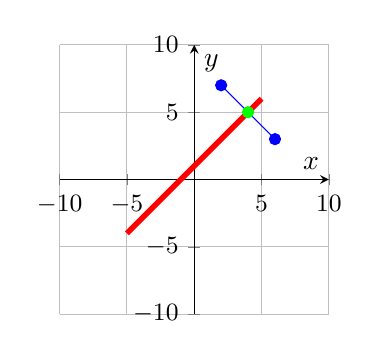
\begin{tikzpicture}[]
					\begin{axis}[width=5cm,height=5cm, axis background/.style={fill=white}, axis lines=middle, 
					grid = major,
					xlabel=$\small x$,
					ylabel=$\small y$, 
					ymin = -10,
					ymax = 10,
					xmin = -10,
					xmax = 10,
					tick label style={font=\small},
					legend style={font=\small,legend pos=outer north east},]
					\addplot [blue,mark=*] coordinates { (2,7)
						 (6,3) };
					 \addplot [green,mark=*] coordinates { (4,5) };
					\addplot[red, samples=201, line width=2pt]{x+1};	
					\end{axis}
					\end{tikzpicture}
					\end{center}
			\end{bluebox}
		
		\item $A=(-3,5)$ i $B=(0, -3)$
		\begin{bluebox}
			 Cercam el punt mitjà $M=\dfrac{A+B}{2}=(-3/2, 1)$
			
			Calculam el vector $\overrightarrow{AB}=B-A=(3, -8)$, que té com a vector perpendicular $\vec n = (8,3)$. Aquest vector correspon un pendent $m = \dfrac{3}{8}$.
			
			Escrivim l'equació punt-pendent de la mediatriu $y-1 = \dfrac{3}{8} (x+\frac{3}{2})$.
			
			Cercam l'equació general $-6x+16y-25=0$
			
			\begin{center}
				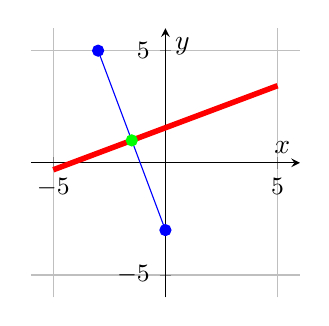
\begin{tikzpicture}[]
				\begin{axis}[width=5cm,height=5cm, axis background/.style={fill=white}, axis lines=middle, 
				grid = major,
				xlabel=$\small x$,
				ylabel=$\small y$, 
				ymin = -6,
				ymax = 6,
				xmin = -6,
				xmax = 6,
				tick label style={font=\small},
				legend style={font=\small,legend pos=outer north east},]
				\addplot [blue,mark=*] coordinates { (-3,5)
					(0,-3) };
				\addplot [green,mark=*] coordinates { (-1.5,1) };
				\addplot[red, samples=201, line width=2pt]{(6*x+25)/16};	
				\end{axis}
				\end{tikzpicture}
			\end{center}
		\end{bluebox}
	
	\newpage
		\item $A=(-1,0)$ i $B=(7,-4)$
		\begin{bluebox}
			Cercam el punt mitjà $M=\dfrac{A+B}{2}=(3, -2)$
			
			Calculam el vector $\overrightarrow{AB}=B-A=(8, -4)$, que té com a vector perpendicular $\vec n = (4,8)$. Aquest vector correspon un pendent $m = \dfrac{8}{4}=2$.
			
			Escrivim l'equació punt-pendent de la mediatriu $y+2 = 2 (x-3)$.
			
			Cercam l'equació general $-2x+y+8=0$
			
			\begin{center}
				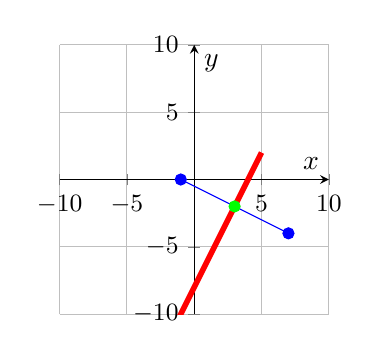
\begin{tikzpicture}[]
				\begin{axis}[width=5cm,height=5cm, axis background/.style={fill=white}, axis lines=middle, 
				grid = major,
				xlabel=$\small x$,
				ylabel=$\small y$, 
				ymin = -10,
				ymax = 10,
				xmin = -10,
				xmax = 10,
				tick label style={font=\small},
				legend style={font=\small,legend pos=outer north east},]
				\addplot [blue,mark=*] coordinates { (-1,0)
					(7,-4) };
				\addplot [green,mark=*] coordinates { (3,-2) };
				\addplot[red, samples=201, line width=2pt]{2*x-8};	
				\end{axis}
				\end{tikzpicture}
			\end{center}
		\end{bluebox}
	\end{enumerate}



	\item[{\Large \bf 36.}] Determina les bisectrius de les rectes r i s. Representa-ho gràficament.
	
	\begin{enumerate}
		\item $r:$ $x+2y-5=0$ i $2x-y-8=0$
		\begin{bluebox}
			\begin{center}
				Si $X(x,y)$ és un punt qualsevol de la bisectriu, ha de complir que 
				\[ dist(X,r) = dist(X,s) \]
				\[ \dfrac{|x+2y-5|}{\sqrt{1^2+2^2}}= \dfrac{|2x-y-8|}{\sqrt{2^2+(-1)^2}} \]
				\[ \dfrac{|x+2y-5|}{\sqrt{5}}= \dfrac{|2x-y-8|}{\sqrt{5}} \]
				\[ |x+2y-5|= |2x-y-8| \]
				\[ \left\{\begin{array}{lcl} x+2y-5= 2x-y-8 & \rightarrow & -x+3y+3=0\\  x+2y-5=-(2x-y-8) & \rightarrow & 3x+y-13=0    \end{array}\right.  \]
				
				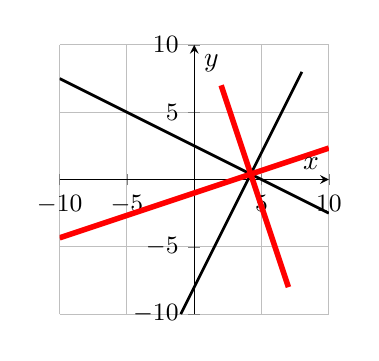
\begin{tikzpicture}[]
				\begin{axis}[width=5cm,height=5cm, axis background/.style={fill=white}, axis lines=middle, 
				grid = major,
				xlabel=$\small x$,
				ylabel=$\small y$, 
				ymin = -10,
				ymax = 10,
				xmin = -10,
				xmax = 10,
				tick label style={font=\small},
				legend style={font=\small,legend pos=outer north east},]
				\addplot[black, samples=201, line width=1pt, domain=-10:10]{(-x+5)/2};	
				\addplot[black, samples=201, line width=1pt, domain=-1:8]{2*x-8};	
				\addplot[red, samples=201, line width=2pt, domain=2:7]{-3*x+13};	
				\addplot[red, samples=201, line width=2pt, domain=-10:10]{x/3-1};	
				\end{axis}
				\end{tikzpicture}
			\end{center}
		\end{bluebox}
	
	\newpage
		\item $r:$ $3x+5y-2=0$ i $4x-6y-1=0$
		\begin{bluebox}
			\begin{center}
				Si $X(x,y)$ és un punt qualsevol de la bisectriu, ha de complir que 
				\[ dist(X,r) = dist(X,s) \]
				\[ \dfrac{|3x+5y-2|}{\sqrt{3^2+5^2}}= \dfrac{|4x-6y-1|}{\sqrt{4^2+(-6)^2}} \]
				\[ \dfrac{|3x+5y-2|}{\sqrt{34}}= \dfrac{|4x-6y-1|}{\sqrt{52}} \]
				\[ \sqrt{52} \,|3x+5y-2|= \sqrt{34}\, |4x-6y-1| \]
				\[ \left\{\begin{array}{lcl}\sqrt{52}\, (3x+5y-2)= \sqrt{34} \, (4x-6y-1) & \rightarrow &  y=-42.02x+19.93\\  \sqrt{52}\, (3x+5y-2)= -\sqrt{34}\, (4x-6y-1) & \rightarrow &  y=0.02x+0.12  \end{array}\right. \]
				
				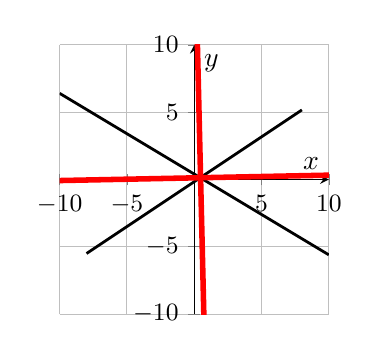
\begin{tikzpicture}[]
				\begin{axis}[width=5cm,height=5cm, axis background/.style={fill=white}, axis lines=middle, 
				grid = major,
				xlabel=$\small x$,
				ylabel=$\small y$, 
				ymin = -10,
				ymax = 10,
				xmin = -10,
				xmax = 10,
				tick label style={font=\small},
				legend style={font=\small,legend pos=outer north east},]
				\addplot[black, samples=201, line width=1pt, domain=-10:10]{(-3*x+2)/5};	
				\addplot[black, samples=201, line width=1pt, domain=-8:8]{(4*x-1)/6};	
				\addplot[red, samples=201, line width=2pt]{-42.02*x+19.93};	
				\addplot[red, samples=201, line width=2pt, domain=-10:10]{0.02*x+0.12};	
				\end{axis}
				\end{tikzpicture}
			\end{center}
		\end{bluebox}
	
	\end{enumerate} 


\item[{\Large \bf 38.}] Donat el triangle de vèrtexs ABC, essent $A=(0,0)$, $B=(6,0)$ i $C=(4,4)$ determina les equacions de:


\begin{enumerate}
	\item Les seves mediatrius i el circumcentre
	
	\begin{bluebox}
		El punt mitjà del segment AB és (3,0) i la recta és vertical, llavors la primera mediatriu és $x=3$.
		
		Anem ara a calcular la mediatriu de BC. El punt mitjà d'aquest segment és $M=(5,2)$. El vector director BC és $(-2,4)$ amb la qual cosa el vector normal és $(4,2)$ i això vol dir un pendent de $m=2/4=1/2$.
		
		La mediatriu BC és per tant $y-2=\frac{1}{2}(x-5)$.
		
		El circumcentre ve de resoldre el sistema d'equacions
		\[ \left\{\begin{array}{l}  y-2=\frac{1}{2}(x-5) \\ x=3  \end{array} \right. \rightarrow  O(1,3)   \]
		
		\begin{center}
		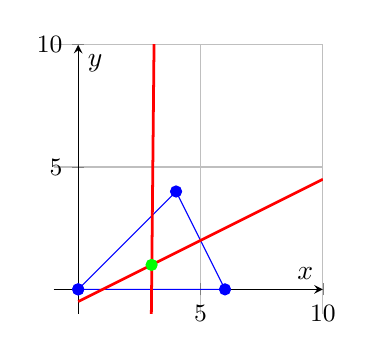
\begin{tikzpicture}[]
		\begin{axis}[width=5cm,height=5cm, axis background/.style={fill=white}, axis lines=middle, 
		grid = major,
		xlabel=$\small x$,
		ylabel=$\small y$, 
		ymin = -1,
		ymax = 10,
		xmin = -1,
		xmax = 10,
		tick label style={font=\small},
		legend style={font=\small,legend pos=outer north east},]
		\addplot [blue,mark=*] coordinates { (0,0)	(6,0) (4,4) (0,0)};
		\addplot[red, samples=201, line width=1pt ]{100*(x-3)};	
		\addplot[red, samples=201, line width=1pt, domain=0:10 ]{2+(x-5)/2};	
		\addplot [green,mark=*] coordinates { (3,1)};
		\end{axis}
		\end{tikzpicture}
	\end{center}
	\end{bluebox}



\item Les bisectrius i l'incentre

\begin{bluebox}
Per calcular les bisectrius primer necessitam calcular les equacions de les rectes de tots els costats.

La recta $r$:  $AB$ és $y=0$

La recta $s$: $AC$ és $x-y=0$

La recta $t$: $CB$ és $2x+y-12=0$

Ara cercam la bisectriu de les rectes $r$ i $s$
	
 \[ \dfrac{|y|}{1}=\dfrac{|x-y|}{\sqrt{2}} \]
 
 Donat que necessitam la bisectiu interior al triangle, agafam el signe correcte que en aquest cas és $+$ (això ho sabem perquè la recta ens ha de sortir creixent).
 
 \[ \sqrt{2} y= +(x-y) \rightarrow  y=0.41x \]
 
	
Ara cercam la bisectriu de les rectes $r$ i $t$

\[ \dfrac{|y|}{1}=\dfrac{|2x+y-12|}{\sqrt{5}} \]

Donat que necessitam la bisectiu interior al triangle, agafam el signe correcte que en aquest cas és $-$ (demanam que la recta sigui decreixent).

\[ \sqrt{5} y= -(2x+y-12) \rightarrow  y=-0.62x+3.7 \]


	
	
	L'incentre s'obté de resoldre el sistema d'equacions
	\[ \left\{\begin{array}{l} y=0.41x  \\y=-0.62x+3.7  \end{array} \right. \rightarrow  I(3.6, 1.5)   \]
	
	\begin{center}
		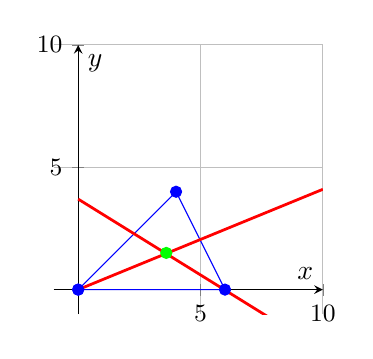
\begin{tikzpicture}[]
		\begin{axis}[width=5cm,height=5cm, axis background/.style={fill=white}, axis lines=middle, 
		grid = major,
		xlabel=$\small x$,
		ylabel=$\small y$, 
		ymin = -1,
		ymax = 10,
		xmin = -1,
		xmax = 10,
		tick label style={font=\small},
		legend style={font=\small,legend pos=outer north east},]
		\addplot [blue,mark=*] coordinates { (0,0)	(6,0) (4,4) (0,0)};
		\addplot[red, samples=201, line width=1pt, domain=0:10 ]{0.41*x};		
		\addplot[red, samples=201, line width=1pt, domain=0:10 ]{-0.62*x+3.7};
		\addplot [green,mark=*] coordinates { (3.6,1.5)};
		\end{axis}
		\end{tikzpicture}
	\end{center}
\end{bluebox}



\item Les altures i l'ortocentre

\begin{bluebox}
	L'altura al costat AB és una recta vertical que passa pel vertex C, és a dir $x=4$.
	
	Anem a calcular l'altura al costat BC. Per això cercam el vector normal a aquesta direcció $\vec n = (4, 2)$, que duu a un pendent de $m=1/2$. La recta que cercam ha de tenir aquest pendent i ha de passar pel punt $A(0,0)$, és a dir
	\[ y = \frac{1}{2}x \]
	
	  
	L'otrocentre s'obté de resoldre el sistema d'equacions
	\[ \left\{\begin{array}{l} x=4  \\y=\frac{1}{2}x  \end{array} \right. \rightarrow  H(4, 2)   \]
	
	\begin{center}
		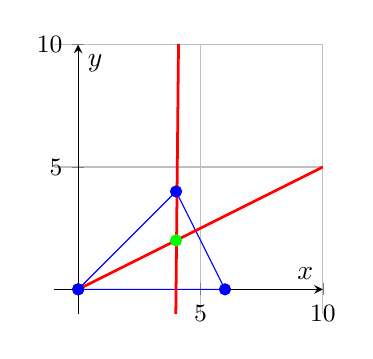
\begin{tikzpicture}[]
		\begin{axis}[width=5cm,height=5cm, axis background/.style={fill=white}, axis lines=middle, 
		grid = major,
		xlabel=$\small x$,
		ylabel=$\small y$, 
		ymin = -1,
		ymax = 10,
		xmin = -1,
		xmax = 10,
		tick label style={font=\small},
		legend style={font=\small,legend pos=outer north east},]
		\addplot [blue,mark=*] coordinates { (0,0)	(6,0) (4,4) (0,0)};
		\addplot[red, samples=201, line width=1pt, domain=0:10 ]{x/2};		
		\addplot[red, samples=201, line width=1pt]{100*(x-4)};
		\addplot [green,mark=*] coordinates { (4,2)};
		\end{axis}
		\end{tikzpicture}
	\end{center}
\end{bluebox}


\item Les medianes i el baricentre

\begin{bluebox}
	La mediana al costat AB és una recta que passa pel punt mitjà $M(3,0)$ i que passa pel vertex C: $y=4(x-3)$
	
	Ara cercam la mediana del costat BC. És una recta que passa pel punt mitjà $M(5,2)$ i que passa pel vertex $A(0,0)$: $y=\frac{2}{5}x$
	
	El baricentre s'obté de resoldre el sistema d'equacions
	\[ \left\{\begin{array}{l} y=4(x-3) \\y=\frac{2}{5}x  \end{array} \right. \rightarrow  G(10/3, 4/3)   \]
	
	\begin{center}
		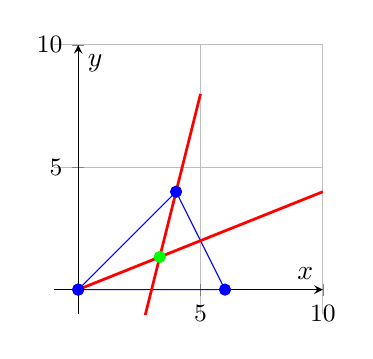
\begin{tikzpicture}[]
		\begin{axis}[width=5cm,height=5cm, axis background/.style={fill=white}, axis lines=middle, 
		grid = major,
		xlabel=$\small x$,
		ylabel=$\small y$, 
		ymin = -1,
		ymax = 10,
		xmin = -1,
		xmax = 10,
		tick label style={font=\small},
		legend style={font=\small,legend pos=outer north east},]
		\addplot [blue,mark=*] coordinates { (0,0)	(6,0) (4,4) (0,0)};
		\addplot[red, samples=201, line width=1pt  ]{4*(x-3)};		
		\addplot[red, samples=201, line width=1pt, domain=0:10]{2*x/5)};
		\addplot [green,mark=*] coordinates { (10/3,4/3)};
		\end{axis}
		\end{tikzpicture}
	\end{center}
\end{bluebox}

\end{enumerate}
\end{mylist}


\end{document}